\documentclass[letterpaper,11pt,openany]{book}
\usepackage[centertags]{amsmath}
%\usepackage[pdflatex]{fullbib-bibtex}
\usepackage{graphicx,amsfonts,amssymb,amsthm,newlfont,macros}
\usepackage{tikz}
\usepackage{float}
\usepackage{graphics}
\usepackage{caption}
\usepackage{hyperref}
\usepackage{booktabs}
\usepackage{tabularx}

\usetikzlibrary{shapes.geometric, arrows}

\newcommand\mat[1]{\boldsymbol{#1}}
\newcommand\vect[1]{\boldsymbol{#1}}
\newcommand\eul{\textup{e}}
\newcommand\imag{\textup{i}}
\makeatletter
% Don't think these are needed so commented them out
%\let\@vwritefile\@writefile
%\def\@ADL@backpage#1{\trelax}
%\newif\ifmtcsecondpart
\@input{classical-control.bux}
\makeatother
\title{MTHE 393 Lab Manual}
\date{\today}
\sloppy 
\begin{document}
\maketitle
\tableofcontents

\chapter*{MTHE 393 Project Intro}\label{chap:Preface_393}


\tikzstyle{startstop}=[rectangle,rounded  corners, minimum width = 4cm, minimum height = 1cm, text centered, draw=black,  fill  = white]
\tikzstyle{arrow1} = [thick,<->,>=stealth]
\tikzstyle{arrow2} = [thick,->,>=stealth]


MTHE 393 consists of two components: a lab component, and a project component. It is the goal 
of the first four labs in this manual to teach you the skills and concepts necessary to successfully 
complete your project. 

\begin{tabular}{p{4cm} p{10cm}}
\vspace{0pt}

\begin{tikzpicture}[node distance = 2cm]
\node (start) [startstop] {1. Experiments};
\node (step1) [startstop,below of = start] {2. Bode Plots};
\node (step2) [startstop, below of = step1] {3. Frequency Resp.};
\node (step3) [startstop,below of  = step2, yshift = -1.5cm] {4. Transfer Function};
\node (step4) [startstop, below of = step3, yshift = -1.75cm] {5. System Dynamics};
\draw[arrow2](start)--(step1);
\draw[arrow1](step1)--(step2);
\draw[arrow1](step2)--(step3) node[midway,right, rotate = 270,xshift = -1.3cm, yshift = 0.25cm]{Freq. Domain};
\draw[arrow1](step3)--(step4) node[midway,right, rotate = 270,xshift = -1.4cm, yshift = 0.25cm]{Laplace Trans.};
\end{tikzpicture}
\captionof{figure}{Project Outline}
\label{Process}


&
\vspace{0pt}
The project itself is fairly straightforward. Teams of students will 
be given a simulated ``Black Box" system, and it will be your job to design a 
controller that will control the outputs of this system, given a set of performance 
specifications. Figure ~\ref{Process} gives a general outline for the 
steps you will be required to take in order to successfully do this. The techniques 
you will learn in these labs will be useful for your project. 
\begin{enumerate}
\item In lab~\ref{chap:freqresp} you will be conducting experiments on the DC motor by 
applying various voltages and measuring the difference between the desired input, and the 
actual output (in this case, the outputs will be angular position and angular velocity of the motor). 
These will give you the necessary information to construct what is called a Bode plot. 
\item A Bode plot is a graph of a systems frequency response. More specifically, several sinusoids 
of varying frequencies will be inputted into the system, then the magnitude and phase difference 
of the desired input vs the actual output will be measured, and plotted on a logarithmic scale. 
These plots are in the frequency domain, therefore they are plots of frequency ($\omega$) 
vs magnitude ($dB$), or frequency ($\omega$) vs phase difference ($rads$).
\end{enumerate}
\end{tabular}
\begin{enumerate}
	\setcounter{enumi}{2}
\item Once you have both Bode plots (magnitude and phase), it is then possible to determine 
your systems frequency response. The frequency response is in the form of a polynomial with various poles and zeros 
in the complex plane. The general shape of a Bode plot is dependent on the number of poles and zeros, 
and their location in the complex plane. Therefore, it is possible to determine the frequency response from 
your experimental bode plots. 
\item The transfer function of a system is what relates the inputs and outputs. If the dynamics of your system are unknown, 
then you have what is called a \emph{Black Box System}. When given a black box system, the transfer 
function is unknown, and you will want to determine an accurate model for it so that you can begin to control the 
system. To determine the transfer function from the frequency response, you must simply substitute the Laplace variable 
$s$ in place of $j\omega$.
\item The dynamics of a given system are typically given by some differential equation. See equation~\ref{eq:motor} 
for the governing equation of the DC motor you will be using in the labs. To find a transfer function for this system, you 
need to work in the \emph{Laplace} domain. This is done by creating  a variable $s=j\omega$, and taking the 
Laplace transform. You may want to review your notes from MTHE 237 on this topic. Once you have taken the 
Laplace transform, you can assess the open-loop stability of the system, and the frequency response. \\
Similarly, you can recover the governing equation of the system from the transfer function by simply taking 
the inverse Laplace transform. For your project, it is at this point that you will begin designing your controller. 
\end{enumerate}
Note that this intro may not be completely clear right away. You may find that as you work through the labs, and 
attend the weekly tutorials that the material will make more sense. This will also be a helpful reference guide 
throughout the project. 

\chapter{Introduction to lab equipment}\label{chap:intro}

The purpose of this lab is to introduce the computer programs and the
equipment you will be using in this course.  You will simulate the operation
of an open-loop motor scheme, illustrated in Figure~\ref{fig:openLoop1}\@.
\begin{figure}[htbp]
\centering
\begin{picture}(200,50)
\put(0,22){$u(t)$}
\put(20,25){\vector(1,0){30}}
\put(55,5){\framebox(105,40)
{\large\((\frac{d^2}{dt^2}+\frac{1}{\tau}\frac{d\theta}{dt})=k_Eu\)}}
\put(165,25){\vector(1,0){30}}
\put(196,22){\(\theta(t)\)}
\end{picture}
\caption{Open-loop motor schematic}\label{fig:openLoop1}
\end{figure}%
Hence, the differential equation governing the system is:
\begin{equation}\label{eq:motor}
\frac{d^{2}\theta}{dt^{2}}+\frac{1}{\tau}\frac{d\theta}{dt}=k_Eu.    
\end{equation}
We are interested in the angle, $\theta$\@, and the angular velocity,
$\omega=\frac{d\theta}{dt}$\@, of the motor shaft.  By the end of the lab,
you will have enough data to calculate the motor time constant, $\tau$\@, and
torque constant, $k_{E}$\@.

\section{Key Concepts}
As the first lab is primarily used to have students familiarize themselves with 
laboratory equipment, it does not focus heavily on course related material. 
However, this lab will introduce you to certain applications of Matlab and Simulink 
which will be used continuously throughout all 9 labs in this manual. Simulink is a 
program that allows us to simulate a system, define an input to this system, 
and send the systems output to Matlab. In these labs our system will be a DC motor, 
to which we will be applying various inputs and observing the outputs. Simulink will 
also be used continuously throughout the project portion of the course. 

\noindent You will be using Matlab throughout this course, so start using some best practices. Some useful tips:
\begin{enumerate}
\item \emph{Always} start a script. Whether you are trying to generate plots, simulate dynamics, or do calculations, it is significantly easier to edit, re-use, re-run code in a script as opposed to the workspace.
\item Save your Simulink models to the cloud. This will save you from having the rebuild your model each week.
\item Use a semicolon ``;" to surpress outputs.
\item You can create Section in your script using double percent signs.
\item The \verb|plot| function can handle multiple $x,y$-tuples. Use this to your advantage. The only requirement is that each vector pair has to be the same \emph{length}. You can have multiple $y$ values for one $x$ vector.
\end{enumerate}
\section{Prelab}

It is assumed that the students of this course will have working knowledge of
personal computers. Before you go into the lab, you should read the
following:
\begin{itemize}
\item Appendix~\ref{chap:MATLAB}\@: \textsf{Matlab}\@;
\item Appendix~\ref{chap:hardware}\@: Lab equipment;
\item Appendix~\ref{chap:simulink}\@: \textsf{Simulink}\@;
\item Section 1.2 from the course text.
\end{itemize}

\noindent Before the lab, you must solve the ODE given in Equation~\ref{eq:motor}, for a constant input $u(t)=1$, using an appropriate technique. 
Remember that for an equation of the form $\frac{dy}{dt} + P(t)y(t) = Q(t)$, the integrating factor $\mu(t) = e^{\int P(t)dx}$. Or, you can use Laplace Transformations.\\

\noindent You will be expected to be able to look up material in the appendices during
the course of the various labs, so it is best that you be familiar with what
is in them.  If you are already familiar with any of the topics, you may skip
that section.

\section{Procedure}

The following steps should be followed to set up the simulink models to
properly communicate with the hardware.  You should perform the following
steps \emph{before} adding any blocks to your simulink model to avoid
manually configuring each block in your model.  Concerning any check boxes,
if it is not explicitly stated that you should check a box then it
\emph{must} be left unchecked.
\begin{enumerate}
\item Create the directory 
\begin{center}
\verb|C:\Documents and Settings\<Qlink ID>\My Documents\MATLAB|
\end{center} 
if it does not already exist.
\item Start \textsf{Matlab}.
\item Type \verb|simulink| at the prompt.
\item Click \verb|File|$\to$\verb|New|$\to$\verb|Model| to create a new empty
simulink model.
\item Build a \textsf{Simulink} model (the following steps will guide you
through this) as shown in Figure~\ref{fig:lab1}\@.
\begin{figure}[htbp]
\centering
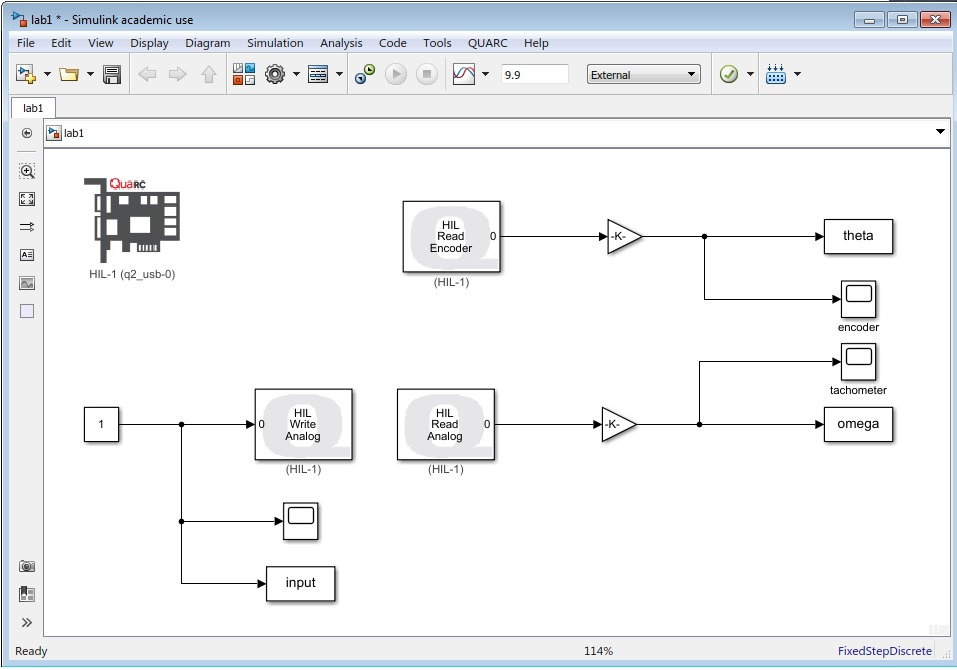
\includegraphics[width=0.9\textwidth]{pix/lab1.PNG} 
\caption{\textsf{Simulink} model for Lab~\ref{chap:intro}}\label{fig:lab1}
\end{figure}%
The model applies a constant voltage to the servomotor.  The encoder is
employed to acquire the angular position ($\theta$) and the tachometer is
used to acquire the angular velocity ($\omega$) as functions of time.
\item Make a new folder on the hard drive under the name or number of your
group and save your model under the name \verb|lab1_name_of_your_group.mdl|.
Save all files created (e.g., model file, plots) in each lab session in that
folder.  It might be a good idea to create a folder for each lab session as
well.

\item Drag the \verb|HIL Initialize| block from the library window into the
model.  You can find this block under:
\begin{center}
\verb|QuaRC Targets|$\to$\verb|Data Acquisition|$\to$\verb|Generic|$\to$\verb|Configuration|
\end{center}
\item Double click on the new \verb|HIL Initialize| block in your model to
configure the parameters.
\begin{enumerate}
\item Main Tab
\begin{itemize}
\item Board Type = \verb|q2_usb|
\end{itemize}
\item Encoder Inputs Tab
\begin{itemize}
\item Encoder Input Channel = \verb|[0]|
\item Encoder Quadrature = \verb|[4]|
\item Encoder Frequency in Hertz = \verb|[ ]|
\item Initial Encoder Counts = \verb|0|
\item Check box \verb|Set encoder input parameters at model start|
\item Check box \verb|Set initial encoder counts at model start|
\end{itemize}
\item Analog Outputs Tab
\begin{itemize}
\item Analog Output Channels = \verb|[0]|
\item Initial Analog Outputs = \verb|0|
\item Final Analog Outputs = \verb|0|
\item Analog Outputs on Watchdog Expiry = \verb|0|
\item Check box \verb|Set initial analog outputs when switching to this model|
\item Check box \verb|Set final analog outputs at model termination|
\item Check box \verb|Set final analog outputs when switching from this model|
\end{itemize}
\end{enumerate}

\item Click \verb|Apply| and then \verb|OK| to close the properties dialog box.

\item Once the \verb|HIL Initialize| block is set up properly, you can add
blocks to your simulink model to read and write analog signals to the
interface board.  The main blocks of interest are \verb|HIL Read Encoder|,
\verb|HIL Read Analog| and \verb|HIL Write Analog|, which replace the old
blocks \verb|Encoder Input|, \verb|Analog Input| and \verb|Analog Output|,
respectively.  Consult the instructions to see which blocks to use in each
lab. There are no \verb|calibration|, \verb|encoder|, or \verb|tachometer|
blocks.  These blocks are simply ``gain'' or ``scope'' blocks which have been
renamed.  It is always best to refer to the block pictures instead of the
block names.  These blocks can be found at
\begin{center}
\verb|QuaRC Targets|$\to$\verb|Data Acquisition|$\to$\verb|Generic|$\to$\verb|Immediate I/0|
\end{center}
\begin{center}
\verb|Simulink|$\to$\verb|Commonly used blocks|
\end{center}
When using the HIL \verb|Read Analog| block, make sure that the correct
channel is set (channel \verb|0|).
\begin{figure}[htbp]
\centering
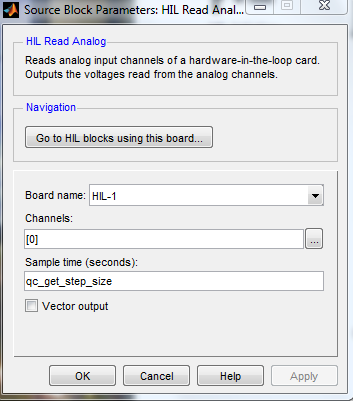
\includegraphics[width=0.5\textwidth]{pix/hil-read-analog-block.PNG}
\caption{HIL \texttt{Read Analog} block settings}\label{fig:hilrab}
\end{figure}
\begin{figure}[htbp]
\centering
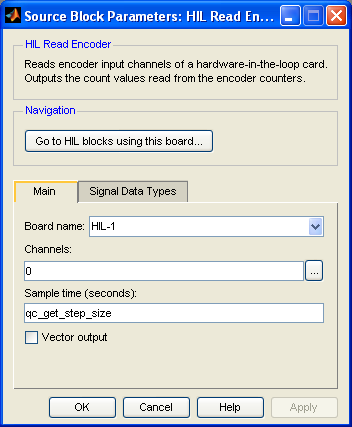
\includegraphics[width=0.5\textwidth]{pix/hil-read-encoder-block.PNG}
\caption{HIL \texttt{Read Encoder} block settings}\label{fig:hilreb}
\end{figure}
\begin{figure}
\centering
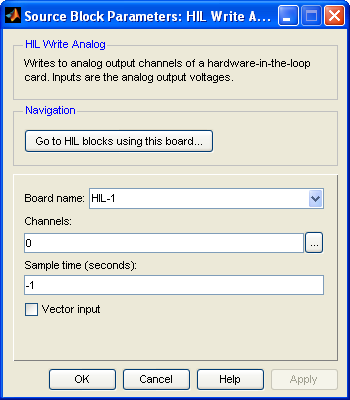
\includegraphics[width=0.5\textwidth]{pix/hil-write-analog-block.PNG}
\caption{HIL \texttt{Write Analog} block settings}\label{fig:hilwab}
\end{figure}
\item The input and output channel numbers in the \textsf{Simulink} blocks should
match the channels used on the terminal board. Refer to
Figures~\ref{fig:hilrab}\@,~\ref{fig:hilreb}\@, and~\ref{fig:hilwab} for the
correct channels.
\item \label{enum:parameters} The calibration factors need to be set so that
servomotor angular position and velocity are acquired in appropriate units. Double
click on the \verb|Gain| block for the encoder and set the gain to $-\frac{2\pi}{4096}$. 
Similarly, set the Tachometer gain to $\frac{100\pi}{63}$. These values can be found in 
Table~\ref{tab:conversionFactors} in Appendix~\ref{chap:hardware}.
\item The \verb|To Workspace| block can be found at
\verb|Simulink|$\to$\verb|Sinks|.  Drag this block into your workspace and
connect it to the variable you wish to save.  Double click on the block to
configure it.  Choose a good variable name and, in the \verb|save format|
drop down menu, select \verb|Structure with time|.
\item Click on \verb|Simulation|$\to$\verb|Configuration Parameters| from
your \textsf{Simulink} screen (or \verb|Ctrl+E|).  Make sure you are using
\verb|fixed-step| integration and choose \verb|ode 4| as your method.  
\item Select \verb|Set default options| from the \verb|QuaRC| drop down menu.
\item Select the \verb|External| mode option from the drop down menu in the toolbar.
Note that \verb|External| mode is only necessary for labs that use the Servomotor. 
\item In the toolbar, change ``inf" to 5 and press enter. This is the simulation time. A note: the software seems to forget all data older than 10 seconds during the simulations, so for the purpose of this lab, we set the \verb|Stop Time| to 5 seconds.
\item Double click on the \verb|Encoder| and \verb|Tachometer| blocks to open
the plots.  More details on viewing real-time results can be found in
Appendix~\ref{chap:simulink}\@.
\item Select \verb|Builld from the \verb|QuaRC| drop down menu.  Wait for
building to be completed before preceding to next step. Progress can be seen
in the Command Window. The keyboard shortcut for building is \verb|Control+B|
\item Provided there are no compilation errors, select
\verb|Connect to Target| from the \verb|Simulation| menu.
\item Select \verb|Run| from the \verb|Simulation| menu, or click
the black play button in the toolbar. The keyboard shortcut for this is \verb|Control+T|.
\item Data will automatically be saved from the \verb|To Workspace| blocks.
\item Plot it with the command
\begin{center}
\verb|plot(varname.time,varname.signals.values)|
\end{center}
replacing ``\verb|varname|'' with the variable name you chose when
configuring the \verb|To Workspace| block.  Use the \verb|plot| command in
\textsf{Matlab} to plot data from the \verb|Encoder| and the
\verb|Tachometer|.  Details on plotting in \textsf{Matlab} are discussed in
Appendix~\ref{chap:MATLAB}\@.  Remember to give the plots appropriate title
and axis labels and print these plots. What is the steady state angular
velocity?  Are the results from these plots as you expected?
\item Now that you have obtained the steady-state value from the angular
velocity plot, you are ready to determine the actual value of the motor time
constant, $\tau$, and the torque constant, $k_{E}$\@.  Recall that solving
the differential equation~(\ref{eq:motor}) with zero initial condition yields
\begin{align}\notag
\omega(t)=&\;\dot\theta(t),\\\label{eq:motorSoln}
\omega(t)=&\;k_{E}\tau (1-e^{-t/\tau}),
\end{align}
and so the steady state value is just $k_{E}\tau$\@.
\item First, determine the steady state value and the constant $\tau$ from
the angular velocity plot.  You can find $\tau$ by using the steady state
value and finding the value of $\omega(t)$ when $t=\tau$\@.
\item Next, determine $k_{E}$ using Equation~(\ref{eq:motorSoln}) and the
constants obtained in the last step.  You might need to zoom in to the
appropriate portion of the graph to see the result clearly.
\item Once you have confirmed with the TA that you have obtained the correct
value of the constants, print a copy of the plot that you zoomed in on.
\item Save all files in the folder you created.  Hand in all the plots you
printed during this lab session and along with it the work to show how you
have obtained the two constants.  Please make sure the names and student
numbers of all your group members are on the first page.
\end{enumerate}
The constants obtained in this lab will come in handy in the future, so make
sure you check with the TA that you have obtained the correct (or reasonably
close) value before you leave.

\textbf{Save your Simulink model to an accessible location. You will need it next week.}

\section{Deliverables}

Prepare a brief write up describing what you learned from this lab. 
This does not need to be a formal report, but all material should be presented in 
a clear and logical manner, with concise descriptions where necessary. Include 
the following/answer the following questions:
\begin{enumerate}
\item Plots of motor position ($\theta$) and velocity ($\omega$) with respect to time. Make sure you label your axes appropriately.
\item What is the steady state angular velocity (in rads/s) of the motor? 
Does this correlate to the value obtained using the encoder plot?
\item Determine the motor constant $\tau$. Include a plot at t = $\tau$ (use proper units).
\item Determine the motor torque constant, $k_E$ (include units). Show your calculations.
\end{enumerate}

%%% Local Variables: 
%%% mode: latex
%%% TeX-master: "lab-manual"
%%% End: 

\chapter{Frequency response and the Bode plot}\label{chap:freqresp}

In this lab you will examine the relationship between the impulse response,
the transfer function, and the frequency response.  You will also compute the
Bode (pronounced ``Boh-dee'') plot of the open-loop motor scheme depicted in
Figure~\ref{fig:openLoop2}\@.
\begin{figure}[htbp]
\centering
\begin{picture}(210,50)
\put(0,20){\(\hat{u}(s)\)}
\put(20,23){\vector(1,0){30}}
\put(55,6.5){\framebox(85,35){\Large\(\frac{k_{E}}{s(s+\frac{1}{\tau})}\)}}
\put(142,23){\vector(1,0){30}}
\put(176,20){\(\hat{\theta}(s)\)}
\end{picture}
\caption{Open-loop motor schematic in frequency domain}\label{fig:openLoop2}
\end{figure}%

\section{Key Concepts}
In this lab we will be determining the relationship between the inputs and outputs 
of a system. Here are a few key topics:
\begin{enumerate}
\item The \emph{Dynamics} of a system govern the input/output relationship
 of a system. These dynamics can be either known, or unknown. In lab~\ref{chap:intro}, 
we observed how our system responded to a simple constant input, however we wish to know 
how it will respond to \emph{all} functions. This is done by observing what is called the 
``Frequency Response" of the system.
\item The  frequency response of a system is determined by first constructing a Bode Plot.  
This is done by inputting different sine waves with varying frequencies, and measuring 
the magnitude and phase difference between the input and the output. For example, 
Figure~\ref{fig:FreqResp} shows the input and output of the system for a sine wave with 
$\omega_u = 5$ rads/sec. Notice how the  magnitude of the output is larger, and the peak time
is shifted by roughly 0.05s. This observation will be made for sine waves with frequencies varying 
from 0.5 rads/sec to 300 rads/sec, or possibly even higher. 
\begin{figure}[htbp]
\centering
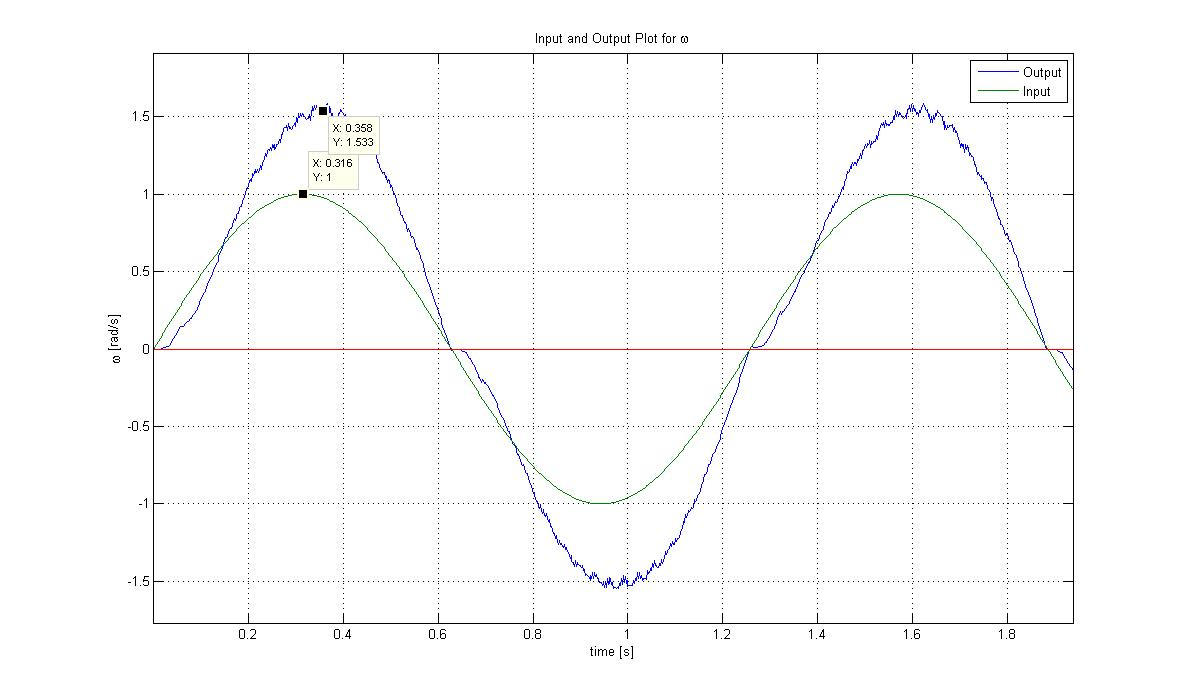
\includegraphics[width=\hsize,height = 0.6\hsize]{pix/FreqResp.jpg}
\caption{\textsf{Matlab} generated plot of the input and output  of the system for $\omega_u = 5$ rads/sec}\label{fig:FreqResp}
\end{figure}

\item Once we have  sufficient data for the magnitude and phase difference, two plots will be created 
(frequency vs. magnitude, and frequency vs. phase angle) using a logarithmic scale. These are your Bode Plots. %reword
\item It is important to remember how these relationships relate to Figure~\ref{Process}. 
In this lab we are conducting experiments as if we did not already know the dynamics of the system. 
This will be how you determine the frequency response of the system you are given for your project,
which will allow you to find a model transfer function for the ``Plant".  


\end{enumerate}

\section{Prelab}\label{sec:prelab4}

\begin{enumerate}
\item Please review Sections 4.1, 4.2, and 4.3 of the course notes for relevant on frequency
response and the production of Bode plots.
\item Compute the Bode plot (by hand) of the motor system when the output is
the motor angle $\theta$.  Recall that the transfer function of that system
is
\begin{equation*}
T(s) =\frac{k_{E}}{s(s+\frac{1}{\tau})}.
\end{equation*}
Use the motor time constant, $\tau$, and the torque constant, $k_{E}$\@,
obtained in Lab~\ref{chap:intro}\@.  Please consult with your TA to make sure
you have the correct values.
\item Repeat the above step when the output is motor velocity $\omega$.
Recall that the transfer function of that system is
\begin{equation*}
T(s) =\frac{k_{E}}{(s+\frac{1}{\tau})}.
\end{equation*}
\end{enumerate}

\section{Procedure}

\subsection{Preliminaries}

In this lab you will be gathering data that will be used to construct the
Bode plot.  Determining the magnitude of the output is straightforward, but
the phase between the input and the output sinusoids is somewhat more
troublesome, but still no match for the wits of seasoned veterans of the
Apple Math program.

To determine the phase difference between two sinusoids, we need to compare
two equivalent points on each sinusoid. Convenient points to consider are
peaks of each sinusoid or where each sinusoid is zero.  Since the magnitude
of each sinusoid can differ, it is more convenient to compare where each
sinusoid is zero. From your plot, measure the time difference between when
the input sinusoid is zero and when the output sinusoid is zero.  Knowing the
time difference and the frequency of the sinusoids, you can use the fact that
$\omega=\frac{d\theta}{dt}=\frac{\Delta\theta}{\Delta t}$ to calculate the
phase difference as $\Delta\theta=\omega\Delta t$\@.

You will find that a good way to organize your data is in a table of the
following format:

\begin{table}[htbp]
\centering
\begin{tabular}{|c|c|c|c|c|c|}\hline
$\omega$&Magnitude&Gain (dB)&Zero-Time Difference&
Phase (rad)&Phase(deg)\\\hline
&&&&&\\
&&&&&\\
&&&&&\\
&&&&&\\
&&&&&\\
\hline

\end{tabular}
\caption{Data collection table}
\label{tab:Data}
\end{table}%



\subsection{MATLAB}

In this part of the lab you will use \textsf{Matlab} to produce the Bode
plots of the mathematical model of the system.

\begin{enumerate}
\item Start \textsf{Matlab} and enter the transfer function corresponding to
each output.  Use the \verb|tf| command to generate the transfer function in
the \textsf{Matlab} command window, then produce the Bode plots of each
transfer function using the \verb|bode| command.

Please refer to Appendix~\ref{chap:MATLAB} on how to use the
\verb|tf| and \verb|bode| command in \textsf{Matlab}.
\item Do not print these plots, but do not close \textsf{Matlab} either.
\end{enumerate}

\subsection{Bode plot}

We will now turn our attention to constructing the Bode plot experimentally,
which we will accomplish by examining the output of the motor given a
periodic input.  The frequency response of a system determines how that
system responds to a harmonic input of frequency $\omega_u$\@.  For this lab,
we will take our harmonic input to be the simple sinusoid $\sin(\omega_u t)$\@.

From your work in Section~\ref{sec:prelab4}, you might guess that
constructing a Bode plot for the motor when the output is the motor angle
will be rather difficult, in which case you would be correct.  However, we
will have a quick look at the angular response of the motor to see if it is
consistent with the Bode plot produced in \textsf{Matlab}.

\begin{enumerate}
\item We begin our exploration of the frequency response with a crude
experiment.  We would like to see what happens over a large range of
frequencies, so we would like $\omega_u$ to increase as $t$ increases.  A
simple way to do this is to define the input function to be $5\sin(t^{2})$\@.
\item Follow Figure~\ref{fig:model4} and build a \textsf{Simulink} model to
implement this signal. \emph{Alternatively, you can modify your model from lab 1}.
\begin{figure}[htbp]
\centering
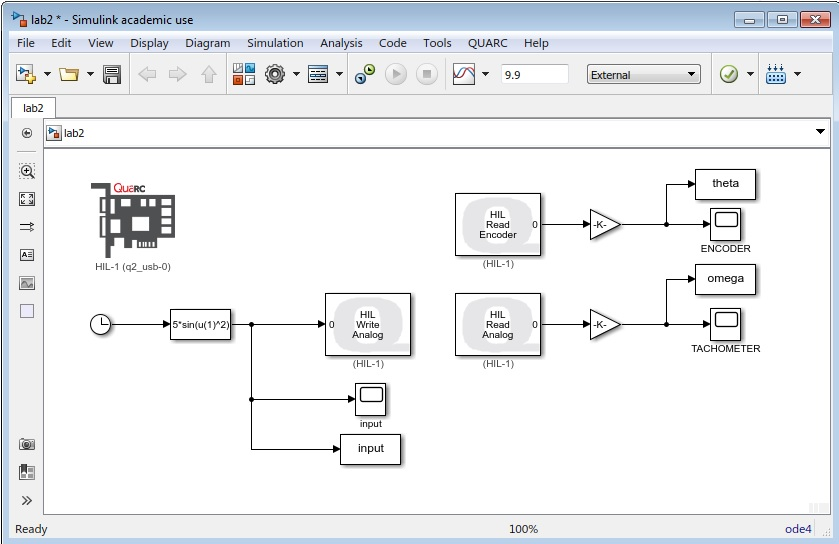
\includegraphics[width=0.6\hsize]{pix/lab2.jpg}
\caption{\textsf{Simulink} model for the implementation of the signal $5\sin(t^{2})$}\label{fig:model4}
\end{figure}%
The \verb|Fcn| block can be found in \textsf{Simulink} in the
\verb|User-Defined Functions| section.  Double-click on your \verb|Fcn| block
to enter the function \verb|5*sin(u(1)^(2))| where \verb|u(1)| represents the
time.  The time is obtained by introducing the \verb|Clock| block as an input
to the function.  The output of the function block is simply connected to the
\verb|Write Analog| block.  Do not forget to change the \verb|solver| to
\verb|ode 4| in \verb|Configuration Paramemters| (\verb|Ctrl+E|). Also,
change the gain constants to the desired units, as in
Step~\ref{enum:parameters} from Lab~\ref{chap:intro}\@. Note: these values can be found in 
Table~\ref{tab:conversionFactors} in Appendix~\ref{chap:hardware}.
\item Change the simulation time in the toolbar to $9.9$~seconds and press enter.
\item \label{enum:simulatet2} Build and run the \textsf{Simulink} model.
Plot the input function $u$, and the output $\theta$ \emph{simultaneously}.
You will notice that $\theta$ is not as well behaved as you might like, but
all you should be concerned with is a rough guess of relative magnitude and
phase with respect to the input function $u$\@.  Does this concur with the
Bode plot you computed with \textsf{Matlab}?  Specifically, comment on the
magnitude and the phase at low and high frequencies.

\item Repeat Step~\ref{enum:simulatet2} but plot the output variable
$\dot\theta$ and $u$ instead of $\theta$ and $u$\@.

\item We will now systematically construct the Bode plot of the motor when
the output is the angular velocity $\omega$ using experimental data. Doing so
will require information about the magnitude and phase of output sinusoid at
various frequencies.  To do this you replace the \verb|Clock| and \verb|Fcn|
blocks by a \verb|Sine Wave| Block.  After you have connected the
\verb|Sine Wave| block to the \verb|Write Analog| block, you can enter the
parameters of the sinusoid you would like to implement.  For the generic
signal, $\sin(\omega_u t)$\@, you may enter the parameters as highlighted in
Figure~\ref{fig:sineConfig}\@.
\begin{figure}[htbp]
\centering
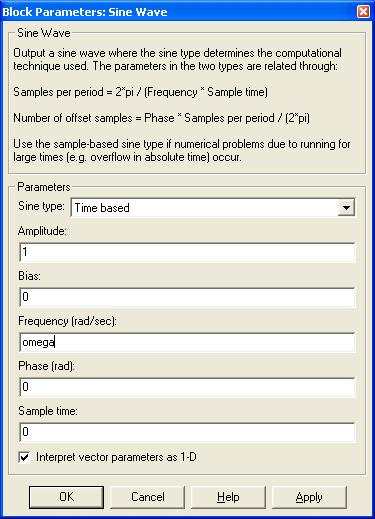
\includegraphics{pix/freqResponseSineConfig.jpg}
\caption{Configuration for the implementation of the signal
$\sin{\omega_u t}$}\label{fig:sineConfig}
\end{figure}%
In this case, the variable \verb|omega|, is undetermined.  The value of
$\omega_u$ must be specified at the \textsf{Matlab} command line before each
run.  The amplitude of $u$ should be set to 1.

\item Build the \textsf{Simulink} model.  For various values of $\omega_u$, run
the system and plot the output variable, $\dot\theta$\@, and the input
variable, $u$\@.  A ``good'' Bode plot can be created using 10--15 well
chosen $\omega_u$ values.  Use the Bode plot generated using \verb|tf| to pick
proper omega values. Note that you do not need to rebuild the \textsf{Simulink} 
model for each new value of $\omega_u$. A good range of $\omega_u$ values would 
be between 0.5 and 300, keeping in mind that this is plotted on a logarithmic scale.%

\item Determine the magnitude of the output sinusoid by recording its peak
amplitude.  It is recommended that you zoom in and out as needed, to ensure a
reasonable degree of accuracy.

\item To determine the phase difference, you will find it most accurate to
look for zero-crossings, as explained above.  You will find that creating an
output variable set to zero is a helpful visual aid in find zero crossings.
Zoom in to accurately observe the time difference when $u$ is zero and when
$\dot\theta$ is zero.  When you are recording the phase differences, you
should be careful that you are recording zero-crossings when both functions are either
increasing or decreasing. This is crucial to keep in mind for higher frequencies.
 This procedure might sound confusing, but usually it is straightforward.%

\item Calculate the phase difference as described in the introduction.

\item With a reasonable amount of data, plot by hand the Bode plot of the
motor when the output is angular velocity, $\omega$. You could also use a
spreadsheet program to organize and plot your data.

When you have completed the lab, make sure you save your files in the folder
you created in the Lab~\ref{chap:intro}\@.
\end{enumerate}

\section{Deliverables}

Prepare a brief write up describing what you learned from this lab. This does not
need to be a formal report, but all material should be presented in a clear and logical manner,
with concise descriptions where necessary. Include the following / answer the following questions:
\begin{enumerate}
\item Include the Matlab generated bode plots for $\theta$ and $\omega$. Use your $k_E$ and $\tau$ values
from lab 1
\item Plots of your motor angular position and velocity compared to the input function $u =  5\sin(t^2)$ (do this on the \emph{same} plot).
Comment on the general trend of the magnitude and phase shift of the outputs. Does this agree
with the bode plots you generated?
\item Include tabulated data from Table~\ref{tab:Data}
\item Include experimental bode plots for both magnitude and phase difference. Ensure the plots \emph{look} like Bode Plots.
\end{enumerate}

%%% Local Variables: 
%%% mode: latex
%%% TeX-master: "lab-manual"
%%% End: 

\chapter{Impulse response and the transfer function}\label{chap:impulseresponse}

In this lab you will be examining the impulse response and the transfer
function of the motor, and the relationship between the two.  Throughout this
lab we will be using the open-loop motor scheme, as depicted in
Figure~\ref{fig:openLoop3}\@,
\begin{figure}[htbp]
\centering
\begin{picture}(200,50)
\put(0,22){$u(t)$}
\put(20,25){\vector(1,0){30}}
\put(55,5){\framebox(105,40)
{\large\((\frac{d^2\theta}{dt^2}+\frac{1}{\tau}\frac{d\theta}{dt})=k_Eu\)}}
\put(165,25){\vector(1,0){30}}
\put(196,22){\(\theta(t)\)}
\end{picture}
\caption{Open-loop motor schematic}\label{fig:openLoop3}
\end{figure}%
but we will be using a constant DC voltage. We will use \textsf{Simulink} to
simulate and implement the system.

\section{Prelab}

The impulse response can be loosely defined as the response of the system to
a ``jolt'' input.  While it is physically impossible to achieve a true
impulse, it is still interesting to study because it reveals much about the
properties of the dynamic system.  Material on impulse response can be found
in Sections 2.4 and 3.5 of the course notes.
 
To make sure that you have a reasonable understanding of the idea of an
impulse response, describe, in words, what happens when a jolt input (a very
short step response) is applied to the motor when: \begin{enumerate} \item
the output is the motor angle, $\theta$; \item the output is the motor
angular velocity, $\omega$. \end{enumerate}

Accompany each with a rough sketch.  You do not have to actually compute
anything, just use your intuition.

\section{Procedure}

\subsection{Impulse Response}\label{cha:impulseRes}

\begin{enumerate}
\item For the open-loop scheme, write out the state equation:
\begin{equation*}
\dot{\vect{x}}=\mat{A}\vect{x}+\vect{b}u,
\end{equation*}
identifying $\vect{x}$\@, $u$\@, $\mat{A}$\@, and $\vect{b}$\@.

\item Determine the output equation:
\begin{equation}
y=\vect{c}^{t}\vect{x}+\mat{D}u,
\end{equation}
identifying $\vect{c}$ and $\mat{D}$ when
\begin{itemize}
\item the output is motor angle, $\theta$\@, and
\item the output is the motor angular velocity, $\omega$.
\end{itemize}

\item Prepare the \textsf{Simulink} model shown in Figure~\ref{fig:model3}.
\begin{figure}[htbp]
\centering
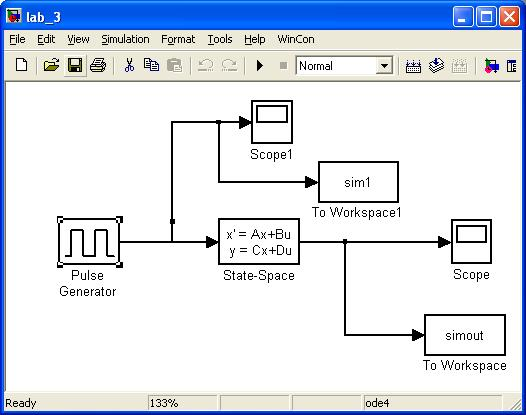
\includegraphics[width=0.6\hsize]{pix/impulseResponseModel.jpg}
\caption{\textsf{Simulink} model for Lab~\ref{chap:impulseresponse}}\label{fig:model3}
\end{figure}%

\item As in Lab~\ref{chap:controlandobserve}\@, enter the motor state
equation using the values of $k_{E}$ and $\tau$ that were estimated in
Lab~\ref{chap:intro} (make sure that you specify the appropriate output).
Double-click on the \verb|Pulse Generator| icon and enter the information as
shown in Figure~\ref{fig:pulseConfig}\@.
\begin{figure}[htbp]
\centering
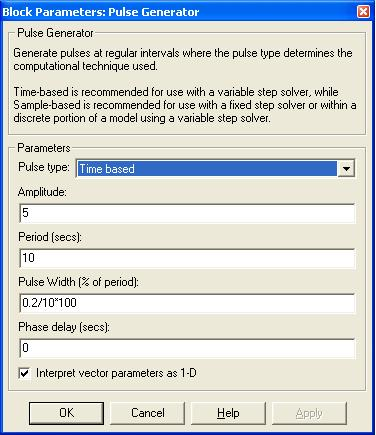
\includegraphics[width=0.6\hsize]{pix/impulseResponsePulseConfig.jpg}
\caption{\texttt{Pulse Generator} configuration for
Lab~\ref{chap:impulseresponse}}\label{fig:pulseConfig}
\end{figure}%
The \verb|Pulse Generator| introduces the impulse function
\begin{equation*}
u_{\epsilon}(t)=\begin{cases}\frac{1}{\epsilon},&
t\leq\epsilon,\\0,&\textrm{otherwise}.\end{cases}
\end{equation*}
every ten seconds.

Recall that the impulse function is defined as
$\lim_{\epsilon\rightarrow0}{u_{\epsilon}}$ (the limit being\ldots er\ldots
in the space of distributions).  Clearly, this is physically impossible to
achieve, but we will approximate as best we can.  The highest voltage that
can be provided by the power supply is 5 volts, so $\epsilon = \frac{1}{5}$
is the lower limit for our system. Pulse width is calculated using the
following formula:
\begin{equation*}
\textrm{Pulse\;Width} = \frac{\frac{1}{\epsilon}}{\textrm{period}}100
\end{equation*}

\item Run the \textsf{Simulink} model. Define the initial conditions to be
zero.  The final time is set to 10 by default.  You may change it by opening
the window
\begin{center}
\verb|Simulation|$\rightarrow$\verb|Configuration Parameters|
\end{center}
and entering the required time in the \verb|Stop time| box.  Start with
$\epsilon=2$ and reduce the value of $\epsilon$ until you see no further
change in the process response.

\item Plot the impulse response for each output described above, using an
appropriate title for each.

\item You will now introduce an impulse into the real system by providing a
``jolt'' by hand. This can be done by tapping the gear.  Prepare the
\textsf{Simulink} model shown in Figure~\ref{fig:model3a}.
\begin{figure}[htbp]
\centering
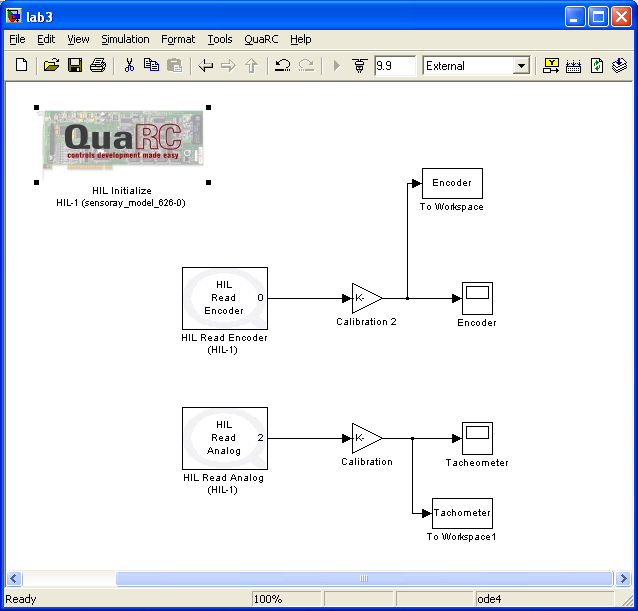
\includegraphics[width=0.6\hsize]{pix/lab3a.jpg}
\caption{Another \textsf{Simulink} model for Lab~\ref{chap:impulseresponse}}\label{fig:model3a}
\end{figure}%
Note that there is no \verb|Write Analog| block required in this case since you are providing the input action.  Using \textsf{Simulink}\@, build the model. Under the Simulation menu, select \verb|Connect to Target|. Then choose \verb|Start Real Time Code|.  Quickly give the motor a ``jolt'' by giving it a quick twist.  Clockwise is taken as the positive direction.

The \verb|Read Encoder| and \verb|Read Analog| parameters are the same as in
Lab~\ref{chap:intro}\@.

\item Plot the response of each state variable while adding an appropriate
title to each plot.

\item Comment on the similarities and differences between the impulse
response and the response of the motor to a hand-powered impulse.

\item To obtain a ``better'' impulse, we introduce the \verb|Pulse Generator|
model as shown in Figure~\ref{fig:model3b}\@.
\begin{figure}
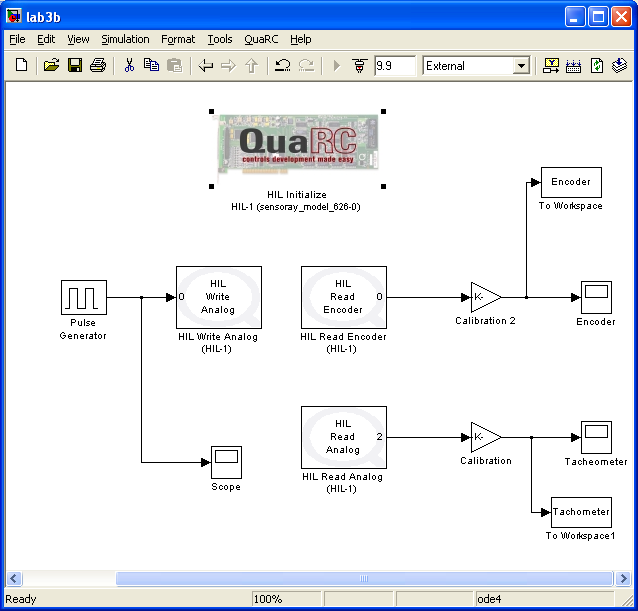
\includegraphics[width=0.9\textwidth]{pix/lab3.PNG} 
\caption{\textsf{Simulink} model for Lab~\ref{chap:impulseresponse}}\label{fig:model3b}
\end{figure}%
Note that the analog output icon has been added since the impulse will be
added automatically in this case.

\item Build and run the model with $\epsilon =1$\@.

\item Run the model again with $\epsilon=\frac{1}{5}$\@.

\item Plot and print the response of the motor angle (encoder input) and the
motor velocity (analog input).  How do these compare with the simulation
impulse response?  With the response due to hand-powered impulse?
\end{enumerate}

\subsection{Transfer Function}

In this part of the lab, you will work in the Laplace transform domain to
analyze this system. Recall that the transfer function $T_{\Sigma}(s)$ is
defined, for example, as the Laplace transform of the impulse response of the
system.
\begin{enumerate}
\item Compute the transfer function from the
standard form, $\dot{\vect{x}}=\mat{A}\vect{x}+\vect{b}u$, $y=\vect{c}^t\vect{x}+\mat{D}u$\@, when
\begin{itemize}
\item the output is the motor angle, $\theta$\@, and
\item the output is the motor angular velocity, $\omega$\@.
\end{itemize}

\item Compute each transfer function again, this time by directly computing
the Laplace transform of the impulse calculated in
Section~\ref{cha:impulseRes}\@.

When you have completed the lab, make sure you save your files in the folder
you created in the Lab~\ref{chap:intro}\@.
\end{enumerate}

%%% Local Variables: 
%%% mode: latex
%%% TeX-master: "lab-manual"
%%% End: 

\chapter{BIBO Stability of systems}\label{chap:stability}

A system is said to be bounded-input, bounded output stable (BIBO stable) if,
given a bounded input, it produces a bounded output. In this lab you will be
using \textsf{Matlab} and \textsf{Simulink} to examine the BIBO stability of
several systems.

\section{Prelab}

Before you go into the lab, you should read the following:
\begin{itemize}
\item Sections 5.1 and 5.2 of the course notes on
system stability.
\end{itemize}

\section{Procedure}

In this part of the lab, you are given three different control systems.  For
each system you will prepare a \textsf{Simulink} model to analyze the outputs
of the system to various bounded inputs, and examine their ``impulse
response'' (even keeping in mind that the true impulse response is a physical
impossibility).
\begin{enumerate}
\item Consider the linear system:
\begin{eqnarray*}
\dot{\vect{x}}&=&\begin{bmatrix}0&1\\-1&0\\\end{bmatrix}\vect{x}
\begin{bmatrix}0\\1\end{bmatrix}u\\
y&=&\begin{bmatrix}1&0\end{bmatrix}\vect{x}
\end{eqnarray*}
and determine $(\mat{A},\vect{b},\vect{c}^{t},\mat{D})$\@.

\item Use the \verb|impulse| command in \textsf{Matlab} to produce the
impulse response of the system (recall that
$h_{\Sigma}(t)=\vect{c}^{t}\eul^{\mat{A}t}\vect{b}$). Comment on the feature
of the impulse response that determines BIBO stability. Do you expect the
system to be BIBO stable?

\item You can calculate the transfer function in several ways: take the
Laplace transform of the impulse response, noting that the systems you are
given are all in controller canonical form; using the \verb|tf| command in
\textsf{Matlab}\@.  Choosing whichever method you like, calculate the
transfer function, and comment on its poles. Is this consistent with your
prediction of BIBO stability?

\item Prepare the \textsf{Simulink} model shown in Figure~\ref{fig:model5}\@.
\begin{figure}[htbp]
\centering
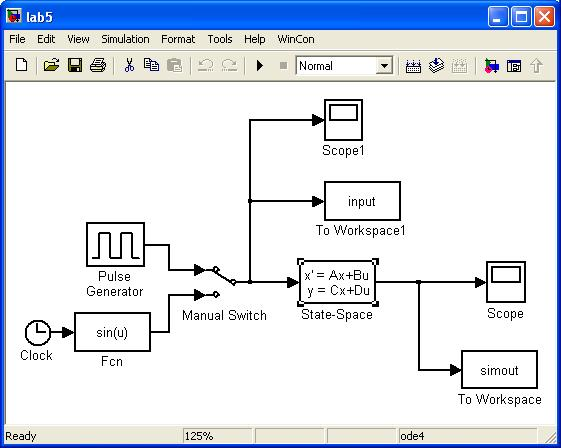
\includegraphics[width=0.6\hsize]{pix/model5.jpg}
\caption{\textsf{Simulink} model for Lab~\ref{chap:stability}}        \label{fig:model5}
\end{figure}%
You could use the model in Lab~\ref{chap:impulseresponse} if you saved it.
They are the same.

\item If you determined that the system is not BIBO stable, modify your
\textsf{Simulink} model by replacing the \verb|Pulse Generator| with the
\verb|Fcn| block and specifying a bounded input that will produce an
unbounded output.  If the system was determined to be BIBO stable, give the
system any bounded input you desire.  In either case, print a plot of the
output variable $y$ and the input variable $u$\@.

\item We will now examine the impulse response of the system.  You can use
the same \textsf{Simulink} model generated above and proceed as in
Lab~\ref{chap:impulseresponse}\@.  Recall that the \verb|Pulse Generator|
block introduced the impulse function
\begin{equation*}
u_{\epsilon}(t)=\begin{cases}\frac{1}{\epsilon},&
t\leq\epsilon,\\0,&\textrm{otherwise}\end{cases}
\end{equation*}
at every specified period.

Run the \textsf{Simulink} model with the initial conditions set to zero.  The
default final time is set to 10s by \textsf{Simulink}\@.  You may change it
by opening the window
\verb|Simulation|$\rightarrow$\verb|Configuration Parameters| and entering
the desired time in the \verb|Stop Time| box.  Larger stop times may be
useful here. Reduce the value of $\epsilon$ until you see no further change
in the process response. Show at least three impulse responses using
different values of $\epsilon$ and note the changes between them.

\item Repeat the procedure for the following two models:
\begin{eqnarray*}
\dot{\vect{x}}&=&\begin{bmatrix}0&1\\-2&-3\\\end{bmatrix}\vect{x}+
\begin{bmatrix}0\\1\end{bmatrix}u\\
y&=&\begin{bmatrix}1&2\end{bmatrix}\vect{x}
\end{eqnarray*}
and
\begin{eqnarray*}
\dot{\vect{x}}&=&\begin{bmatrix}0&1\\4&-3\\\end{bmatrix}\vect{x}+
\begin{bmatrix}0\\1\end{bmatrix}u\\
y&=&\begin{bmatrix}0&1\end{bmatrix}\vect{x}.
\end{eqnarray*}

\item In Lab~\ref{chap:impulseresponse} you examined the impulse response of
the motor system when the output of the system was the motor angle,
$\theta$\@, and the motor velocity, $\omega$\@.  Using the data you gathered
in that lab, comment on the BIBO stability of both systems, commenting on the
impulse response, and poles of the function.

When you have completed the lab, make sure you save your files in the folder
you created in Lab~\ref{chap:intro}\@.
\end{enumerate}

%%% Local Variables: 
%%% mode: latex
%%% TeX-master: "lab-manual"
%%% End: 


\appendix
\chapter{Matlab}\label{chap:MATLAB}

The students of this course should be familiar with the basic ideas of
computer programming and Matlab from first year courses.

\section{Defining variables}

\begin{itemize}
\item \verb|x=3|\\
Defines the variable \verb|x| to be the constant 3.
\item \verb|x=(1,2;3,4;5,6)|\\
Defines the variable \verb|x| to be the $3 \times 2$ matrix
\begin{equation*}
\begin{bmatrix}1&2\\3&4\\5&6\end{bmatrix}
\end{equation*}
Elements of a row are delimited by commas (or spaces) and each row is
delimited by a semicolon.
\end{itemize}

\section{General Commands}

\begin{itemize}
\item \verb|dir|\\
Displays a list of files in the current directory.
\item  \verb|open lab_1.mdl|\\
Opens the specific file in the argument. We will be dealing mostly with
\verb|*.mdl| and \verb|*.m| files.
\item \verb|who|\\
Displays a list of variables in the memory of \textsf{Matlab}.
\item \verb|simulink|\\
Opens the \verb|Simulink Browser Library| window.  Using the GUI control, you
can drag and drop the blocks to build the \textsf{Simulink} models needed for
each lab.  Details on using \textsf{Simulink} and WinCon are discussed in
Appendix~\ref{chap:simulink}.
\end{itemize}

\section{Plotting}

\begin{itemize}
\item \verb|plot (lab_1_Tachometer)|\\
Plots the data from the variable \verb|lab_1_Tachometer| in \textsf{Matlab} memory.
You can check the list of variables in the \textsf{Matlab} memory by using the
\verb|who| command.

\item \verb|plot (lab_1_Tachometer,'r:')|\\
Plots the result in the memory of \textsf{Matlab} and specifies the colour of
the graph to be red and the line style to be dotted.  Colour and line format
are optional commands and they do not have to be specified for the plot
command to produce an output. You can also specify one style parameter
without the other.  The default colour is blue and the default line style is
solid.  Table~\ref{tab:colour} is a list of colours and line styles that can
be used with the plot command.
\begin{table}[htbp]
\centering
\begin{tabular}{|c|c|}\hline
Line style/colour & \textsf{Matlab} command\\\hline
solid & '\verb|-|'\\\hline
dashed &'\verb|--|'\\\hline
dotted & '\verb|:|'\\\hline
dash-dot&'\verb|-.|'\\\hline
blue & '\verb|b|' or '\verb|blue|'\\\hline
black& '\verb|k|' or '\verb|black|'\\\hline
cyan & '\verb|c|' or '\verb|cyan|' \\ \hline
green & '\verb|g|' or '\verb|green|' \\\hline
magenta & '\verb|m|' or '\verb|magenta|' \\ \hline
red & '\verb|r|' or '\verb|red|'\\ \hline
white & '\verb|w|' or '\verb|white|'\\ \hline
yellow &'\verb|y|' or '\verb|yellow|' \\ \hline
\end{tabular}
\caption{Colour commands in \textsf{Matlab}}\label{tab:colour}
\end{table}

\item \verb|title ('Angular Velocity of the Motor')|\\
Sets the title of the plot to the text in quotations.

\item \verb|xlabel ('Time (s)')|\\
Sets the x-axis label of the plot to the text in quotations.

\item \verb|ylabel ('rad/sec')|\\
Sets the y-axis label of the plot to the text in quotations.

\item \verb|hold|\\
Hold the current graph in figure and allow the user to plot more than one set
of data on the same figure.

\item \verb|hold off|\\
Release the current graph in figure and allow a new plot to replace the
current graph.
\end{itemize}

\section{Control System Toolbox}

\begin{itemize}
\item \verb|sys = ss(A,b,c,D)|\\
Defines the the state-space system from matrices $\mat{A}$\@, $\vect{b}$\@,
$\vect{c}$\@, and $\vect{D}$\@.  For a model with $n$ states and $1$ output,
\begin{itemize}
\item $\mat{A}$ is an $n\times n$ matrix,
\item $\vect{b}$ is an $n\times 1$ matrix,
\item $\vect{c}$ is a $1\times n$ matrix ($\vect{c}^{t}$ in our notation),
and
\item $\mat{D}=[0]$ (always true for this class).
\end{itemize}


\item \verb|h = tf([1 0],[1 2 10])|\\
Defines the variable \verb|h| to be the transfer function
\begin{equation*}
\frac{s}{s^{2}+2s+10}.
\end{equation*}

\item \verb|h = zpk([1 0],[-1 -2 -10],[3])|\\
Defines the variable \verb|h| to be the transfer function using the location
of the zeros, poles, and a multiplicative constant:
\begin{equation*}
\frac{3s(s-1)}{(s+1)(s+2)(s+10)}.
\end{equation*}

\item \verb|h = tf(sys)|\\
Defines the variable \verb|h| to be the transfer function for a given
state-space system.

\item \verb|sys = tf2ss[tf]|\\
Gives the SISO linear system corresponding to the transfer function \verb|tf|.

\item \verb|bode(sys)|\\
Produces the Bode plots for the given system.

\item \verb|impulse(sys)|\\
Produces the impulse response for the given system.

\item \verb|nyquist(sys)|\\
Produces the Nyquist plot for the given system.

\item \verb|margin(sys)|\\
Produces the gain and phase margins with associated crossover frequencies.
\end{itemize}

%%% Local Variables: 
%%% mode: latex
%%% TeX-master: "lab-manual"
%%% End: 

\chapter{Simulink}\label{chap:simulink}

\textsf{Simulink} allows simulation of complex control systems using a drag
and drop block diagram interface.  \textsf{Simulink} is especially useful
when used in conjunction with the Real-Time Workshop which allows
\textsf{Simulink} diagrams to be converted into C codes which can be run in
real-time on a number of so-called targets (the PC being one such target).

\section{Starting}

\begin{itemize}
\item To use \textsf{Simulink}, one must first start \textsf{Matlab}.  After
starting \textsf{Matlab}, you would type \verb|simulink| in the
\textsf{Matlab} command prompt to get the \verb|Simulink Library Browser|
window.

\item Selecting \verb|File|$\to$\verb|New|$\to$\verb|Model| (or
\verb|Ctrl+N|) while in the \verb|Simulink Library Browser| will give you a
blank model window into which you can drag-and-drop system blocks from the
\verb|Simulink Library Browser| to build a \textsf{Simulink} model.  These
models can be saved as \verb|*.mdl| files for future simulations and editing.
\end{itemize}

\section{Building a \textsf{Simulink} model}

\begin{itemize}
\item To connect the output of block~A to the input of block~B, simply
left-click the output port of block~A and drag the line that would appear
into the input port of the block~B.

\item In order to connect the output of a block into the inputs of multiple
blocks at the same time, you can right-click on an existing connection to get
another line and drag that connection into the input of another block.

\item When a block is dragged into the model window, it will be given a
generic name.  For example, when the \verb|scope| block is dragged into a
model, it would simply be labelled as ``scope'' and if it was the second
\verb|scope| block to be dragged into the model, it would be labelled as
``scope2''.  It is a good practice to rename these blocks and give them more
appropriate labels.  These names are usually suggested in the diagram of the
models in each lab. To rename a block, simply click on the existing name once
and edit.
\end{itemize}

\section{Simulations}

\begin{itemize}
\item One could view and edit the simulation parameters by clicking on
\begin{center}
\verb|Simulation|$\to$\verb|Simulation Parameters|
\end{center}
(or \verb|Ctrl+E|) while editing the model.  For the purpose of this course,
there are only three things that you have to worry about:
\begin{enumerate}
\item Start and stop time: The default start time is 0 and the default stop
time is 10.  Usually, there is no reason to change the default start time,
but you might find it useful to extend the stop time so that you could
observe the simulation for a longer period of time.

\item Solver Method: You must have this set to a fixed-step when implementing
real-time controllers. The default solver is a discrete method. You need to
change it from the default method to \verb|ode4|, which is an implementation
of the Runge-Kutta method.

\item Step size: The default setting of 0.001 corresponds to 1000 Hz sampling
frequency.  This is the fastest rate at which the system can sample.
\end{enumerate}
\end{itemize}

\section{Plotting}

\begin{itemize}
\item The outputs of a simulation can be captured by using the
\verb|To Workspace| block.  The data would be recorded as a variable in
memory of \textsf{Matlab}.  The default name of the output is \verb|simout|,
but you should change the name of this output just as you would give
appropriate label to the block itself.  One could plot the simulation output
by using plot command discussed in Appendix~\ref{chap:MATLAB}\@.
\end{itemize}

\subsection{Saving data via the ``To Workspace'' block}

This is the preferred method of saving data to your \textsf{Matlab}
workspace.  The \verb|To Workspace| block can be found at
\begin{center}
\verb|Simulink|$\to$\verb|Sinks|
\end{center}
Drag this block into your workspace and connect it to the variable you wish
to save.  Double click on the block to configure it.  Choose a good variable
name and in the \verb|save format| drop down menu select
\verb|Structure with time|.  After the simulation the data will be
automatically saved to your \textsf{Matlab} workspace and you can plot it
with the command
\begin{center}
\verb|plot(varname.time,varname.signals.values)|
\end{center}
replacing ``\verb|varname|'' with the variable name you chose when
configuring the \verb|To Workspace| block.

\subsection{Saving data from a scope}

You can also save scope data, but the scope seems to have short-term memory
loss which makes it one of the most useless blocks in the simulink library.
Nevertheless if you need to save the data from a scope, follow these
instructions.
\begin{enumerate}
\item Double click on the scope you wish to save the data from.
\item Click on the Parameters Icon (in the top left of the scope dialog box).
\item Data History Tab
\begin{itemize}
\item Uncheck box \verb|Limit data points|
\item Check box \verb|Save data to workspace|
\item Choose a variable name
\item Select \verb|Array| from the Format drop down menu.
\end{itemize}
\item Click \verb|Apply| and \verb|OK| to exit.
\end{enumerate}
After the simulation has been performed, the data will appear as an array in
your \textsf{Matlab} workspace.  You can plot the data with the
command \begin{center}
\verb|plot(ScopeData1(:,1), ScopeData1(:,2))|
\end{center}
where \verb|ScopeData1| is the variable name that you set in the above steps.

%%% Local Variables: 
%%% mode: latex
%%% TeX-master: "lab-manual"
%%% End: 

\chapter{Lab Equipment}\label{chap:hardware}

In the lab, there are several computers equipped with data acquisition
systems running Windows~7 with Matlab. The hardware equipment and some
software tools are manufactured by \href{http://www.quanser.com/}{Quanser
    Consulting}, a Canadian company developing real-time control systems for
education and research. This document introduces some of the hardware
equipment to be used in the labs. Familiarity with this document is needed to
perform the labs.

\section{Servomotor (Lab 1)}
\subsection{Hardware devices}

The lab hardware consists of three components:
\begin{enumerate}
    \item data acquisition system;
    \item power module;
    \item servomotors.
\end{enumerate}

\subsection{Data Acquisition Board}

In order for the computer to run a controller, analog-to-digital (A/D) and
digital-to-analog (D/A) conversions are necessary. These are done using the
data acquisition and control board (DACB), which inputs the measured
signal(s) to the computer and outputs control action to the actuator in the %chktex 36
control loop.  The DACB in this lab consists of a single board: the Q2-USB,
which is made by Quanser Consulting.  Figure~\ref{fig:q2usb}
\begin{figure}[htbp]
    \centering
    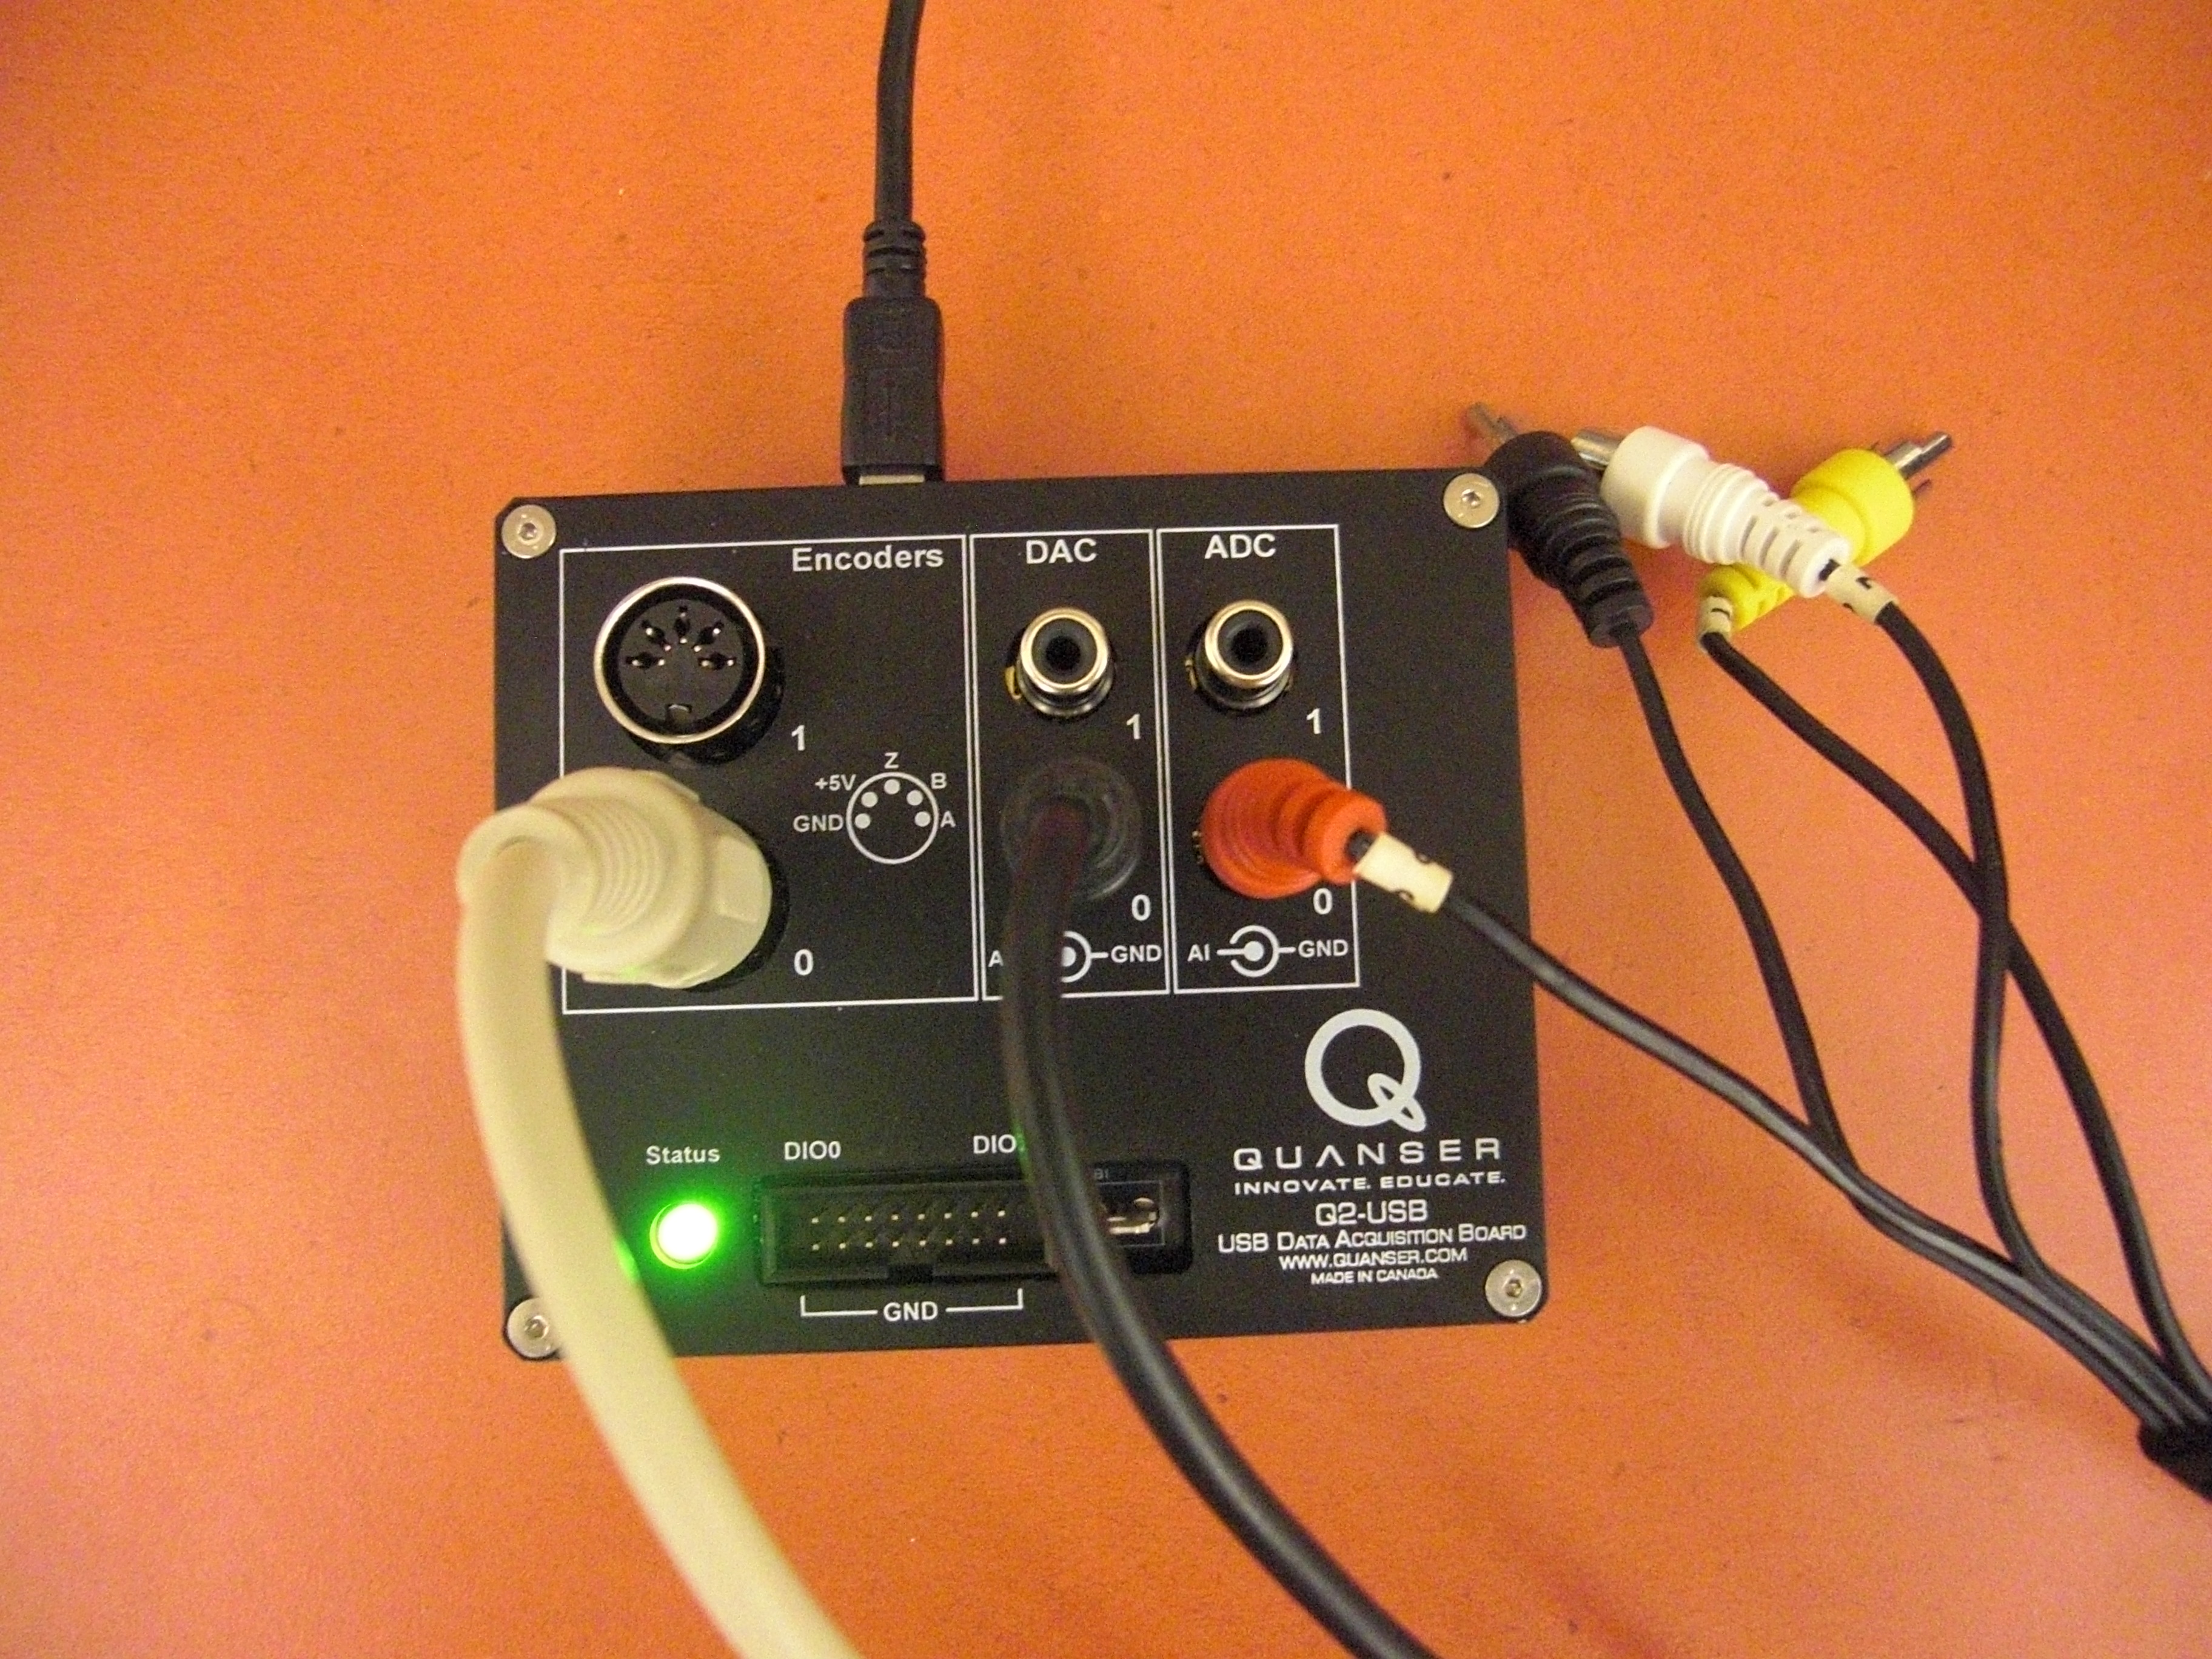
\includegraphics[width=0.6\hsize]{pix/Q2USB.jpg}
    \caption{Q2-USB data acquisition board}\label{fig:q2usb}
\end{figure}%
shows a photo of the Q2-USB card. This data acquisition board is an external
board connected to the computer through a USB port.

Figure~\ref{fig:q2usb} also shows the proper configuration of the data
acquisition board.  The Encoder is the 5~pin Din and is plugged in to
channel~0 in the Encoders portion of the board. The tachometer (S3 on the
Quanser) is the red RCA plug and is plugged into channel~0 is the ADC
portion of the board.  Finally the analog output is the solo black RCA plug
and is plugged in to channel~0 of the DAC portion of the board.

\subsection{Universal power module}

The universal power module (UPM-2405), which is shown in
Figure~\ref{fig:power}\@,
\begin{figure}[htbp]
    \centering
    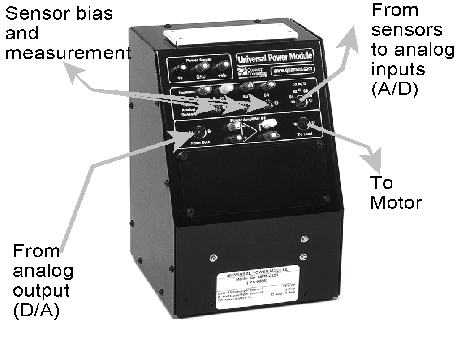
\includegraphics[width=0.6\hsize]{pix/power.jpg}
    \caption{Universal power module}\label{fig:power}
\end{figure}%
is a linear power operations amplifier. The Q2-USB data acquisition board
cannot deliver enough power to the actuators used in this lab; therefore, a
signal buffer is needed.  The UPM-2405 is used as our signal buffer since it
can deliver up to 5A~to an actuator in a non-inverting, unity gain
configuration.

The following connections can be made to/from the UPM (see the labels on the
UPM).
\begin{itemize}
    \item From analog sensors: there are four (S1-S4 inputs which can be
          connected from analog sensors (and then subsequently to the computer); the
          cable used is a 6-pin mini-din/6-pin mini-din cable (light tan colour), which
          is now referred to as the analog sensor cable.

    \item To A/D:\@ the four analog sensor signals (S1-S4) can then be connected to
          the Q2-USB terminal board for A/D conversion into the computer; the cable
          used is a 5-pin din-stereo/4RCA cable (black colour), which is now referred to
          as the A/D cables.

    \item From D/A:/@ this is where you input the D/A signal from the Q2-USB
          terminal board to the UPM;\@ the cable used is a 5-pin din-mono/RCA cable
          (black colour), which is now referred to as the D/A cable.

    \item To load: here you connect the amplified D/A signal to an actuator
          (e.g., servomotor); the cable used is a 7-pin din/4-pin din cable (black
          colour), which is now referred to as the load cable.  Note there are two types
          of load cables one with unity gain and another with a cable gain of 5.  Make
          sure you use the right one.

    \item Others: A few other connections are possible for convenience: e.g., a
          DC power supply on the top left provides 12 volts; the signal s from analog
          sensors S1-S4 can be easily monitored by connecting to a scope to the banana
          plug terminals.
\end{itemize}

\subsection{DC servomotor}

The Quanser DC servomotor (SRV02) is shown in Figure~\ref{fig:motor}\@.  A 3W
motor is mounted in a solid aluminium frame and drives a built-in Swiss-made
14.1:1 gearbox whose output drives an external gear, which is attached to an
independent output shaft that rotates in an aluminium ball-bearing block.
The output shaft is equipped with an encoder.  The external gear on the
output shaft drives an anti-backlash gear connected to a precision
potentiometer for measuring the output angle.  The external gear ratio can be
changed from 1:1 to 5:1 using different gears.  Two inertial loads are
supplied with the system in order to examine the effect of changing inertia
on motor performance.
\begin{figure}[htbp]
    \centering
    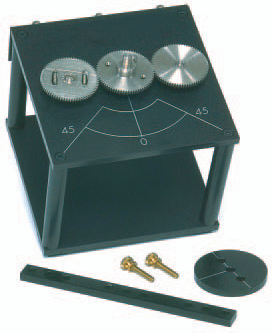
\includegraphics[width=0.6\hsize]{pix/motor-eps-converted-to.pdf}
    \caption{DC servomotor (SRV02)}\label{fig:motor}
\end{figure}%
Several connections are available for the servomotor. The input voltage
connects to the UPM using the load cable.  The potentiometer and tachometer
ports connect to the UPM-2405 using sensor cables and are used to measure
angular position and angular velocity respectively.  Additionally, the shaft
encoder port connects to the terminal board using an encoder cable and is
used to measure angular position.  The calibration factors listed in
Table~\ref{tab:conversionFactors} are needed in order to use the sensors in
units of degrees or radians.

\begin{table}[htbp]
    \centering
    \begin{tabular}{c c c }
        Connection    & Conversion (Rad)                                    & Conversion (Deg)                                   \\\bottomrule
        Encoder       & \(-\frac{2\pi}{4096}\)                              & \(-\frac{360}{4096}\)                              \\
        Tachometer    & \(\frac{100\pi}{63} \frac{\text{rad}}{\text{sec}}\) & \(\frac{18000}{63} \frac{\text{deg}}{\text{sec}}\) \\
        Potentiometer & \(\frac{1}{4096}\)                                  & \(\frac{180}{4096\pi}\)                            \\
    \end{tabular}
    \caption{Conversion factors}\label{tab:conversionFactors}
\end{table}

\section{Rotary Pendulum (Lab 3)}
\subsection{Setting up the Rotary Pendulum}\label{subsection:lab2_setup}
First, let us assemble and wire the physical system. Examine the close-up assembly shown in Figure~\ref{fig:lab1a_assembly}, and replicate this at your workstation. Note that the high-gear configuration is used here. Use the wiring diagram shown in Figure~\ref{fig:lab1a_wiring} to connect the rotary pendulum to a power source and the data acquisition board.
\begin{figure}[htb!]
    \centering
    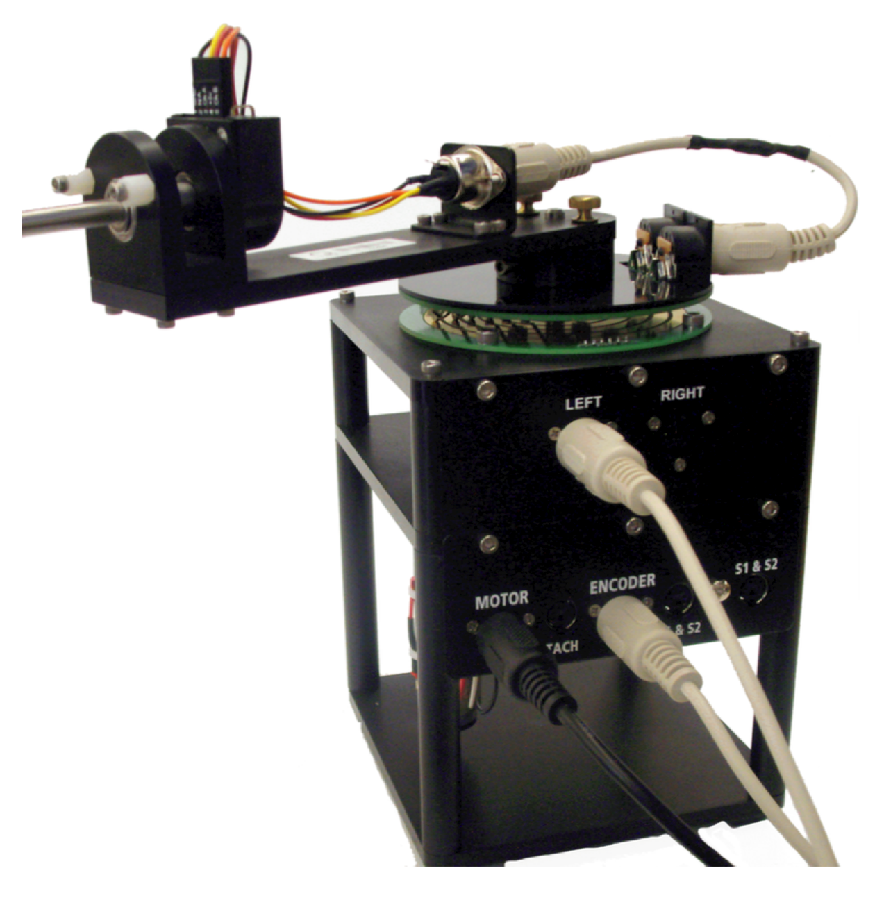
\includegraphics[width=.3\linewidth]{eps/lab_2/assembly.eps}
    \caption{A close-up of the assembly of the rotary pendulum module and the Quanser SRV02 plant~\cite{Q-Flex-Beam}.}
    \label{fig:lab1a_assembly}
\end{figure}
\begin{figure}[htb!]
    \centering
    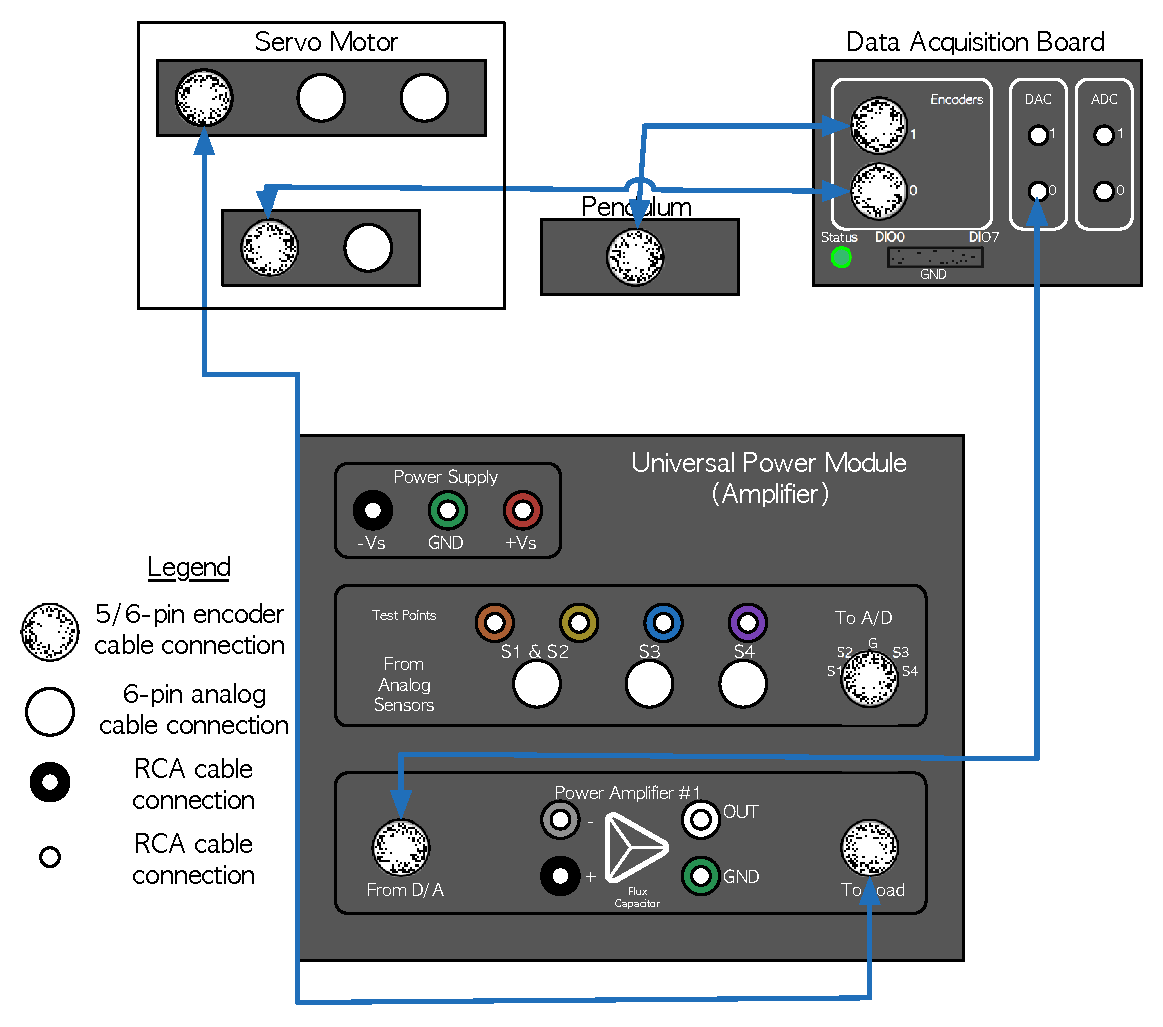
\includegraphics[width=.7\linewidth]{eps/lab_2/wiring.eps}
    \caption{A wiring diagram for the Quanser SRV02 and rotary pendulum module.}
    \label{fig:lab1a_wiring}
\end{figure}

\textbf{Note:} The power amplifier must be turned on before you can experiment with the physical system. The power switch is located at the back of the amplifier (good luck finding it). Make sure to turn off the power amplifier before you leave the lab.

\section{Flexible Beam {Lab 4}}
First, you must assemble and wire the physical system correctly. Examine the close-up assembly shown in Figure~\ref{fig:lab1_assembly} and replicate this at your workstation. Note that the high-gear configuration is used here: a large gear is connected to a small pinion and a slip gear, rather than using the smaller gear. You will need to build a two-tiered gear train as shown in Figure~\ref{fig:lab1_assembly} to make the large gear fit correctly. Use the wiring diagram shown in Figure~\ref{fig:lab1_wiring} to connect the rotary pendulum to a power source and the data acquisition board.
\begin{figure}[htb!]
    \centering
    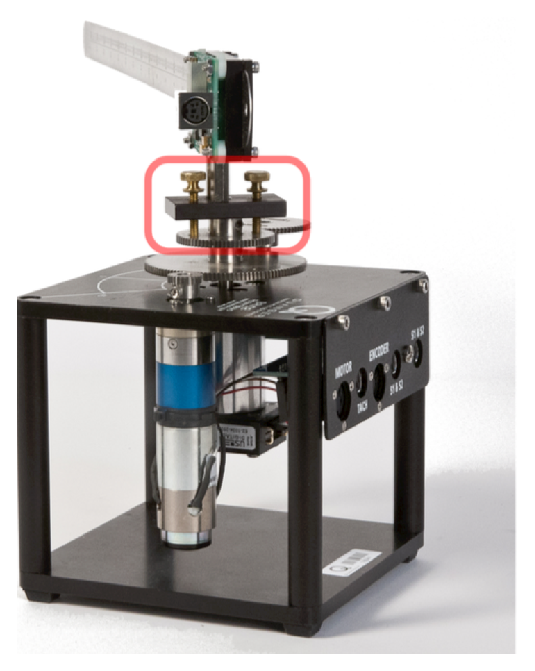
\includegraphics[width=.3\linewidth]{eps/lab_1/assembly.eps}
    \caption{A close-up of the assembly of the rotary flexible beam module and the Quanser SRV02 plant~\cite{Q-Flex-Beam}. The high-gear gear train is indicated by a red box.}
    \label{fig:lab1_assembly}
\end{figure}
\begin{figure}[htb!]
    \centering
    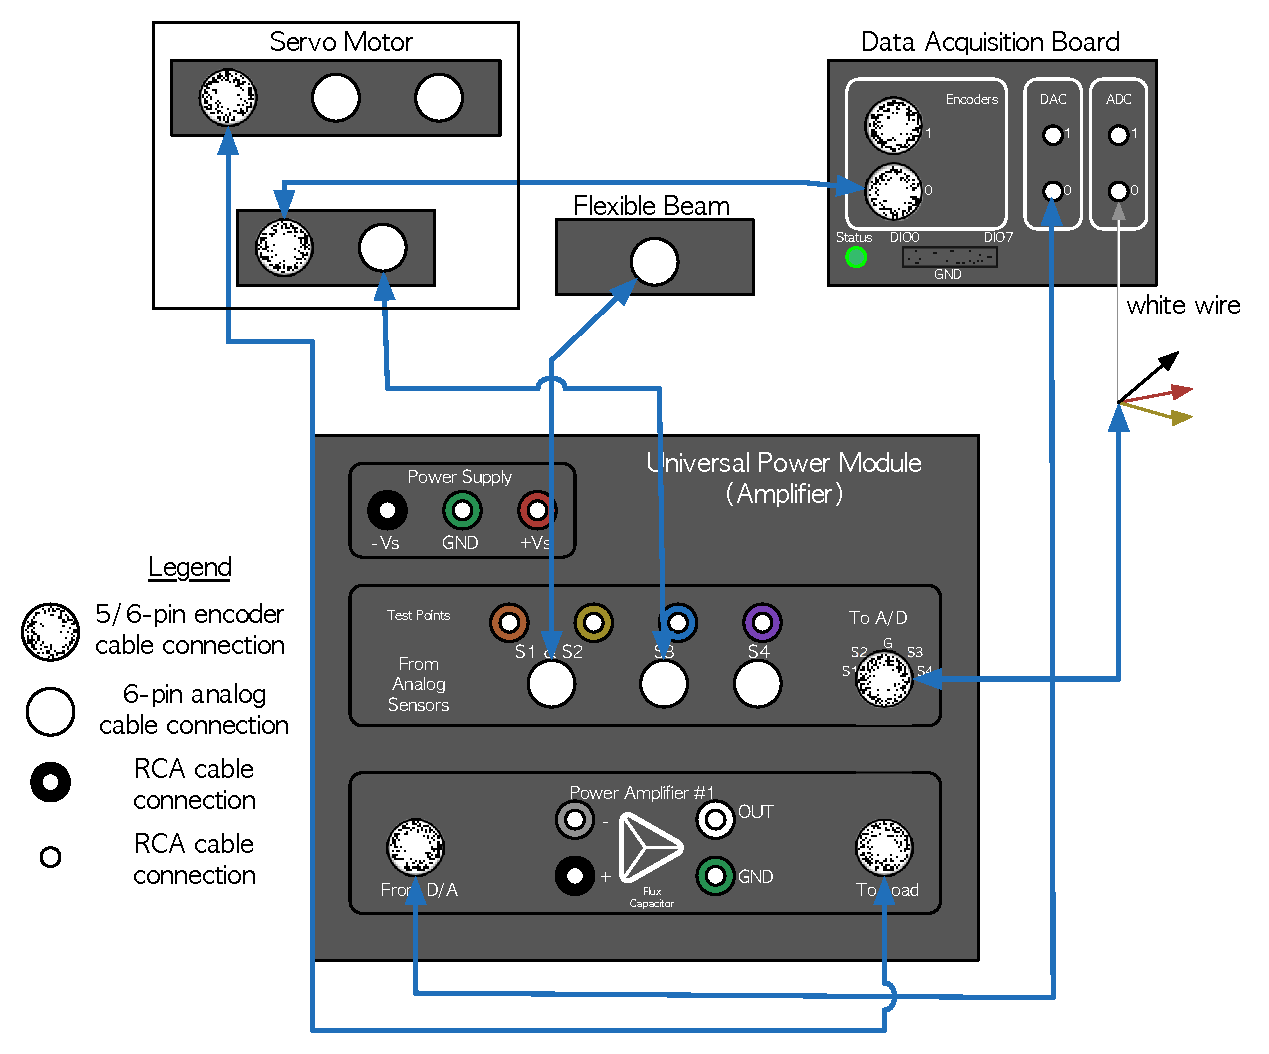
\includegraphics[width=.8\linewidth]{eps/lab_1/wiring.eps}
    \caption{A wiring diagram for the Quanser SRV02 and rotary flexible beam module.}
    \label{fig:lab1_wiring}
\end{figure}

%%% Local Variables: 
%%% mode: latex
%%% TeX-master: "lab-manual"
%%% End: 


\end{document} %chktex 17